% samplepaper.tex: springer.com
% modificato da MM 06/05/2018
%
\documentclass[runningheads]{llncs}
\usepackage[italian]{babel}
\usepackage{graphicx}
\usepackage{subfigure}
% Used for displaying a sample figure. If possible, figure files
% should be included in EPS format.  If you use the hyperref package,
% please uncomment the following line to display URLs in blue roman
% font according to Springer's eBook style:
% \renewcommand\UrlFont{\color{blue}\rmfamily}
\begin{document}
%
\title{Organizzazione e contenuti della relazione di mini-progetto per il gruppo ACC}
%
% \titlerunning{Abbreviated paper title}
% If the paper title is too long for the running head, you can set
% an abbreviated paper title here
%
\author{%
  Alessandro Stefani\inst{1} \and
  Caterina Buranelli\inst{2} \and
  Cristi Gutu\inst{3}}
%
\authorrunning{P. Autore et al.}
% First names are abbreviated in the running head.  If there are more
% than two authors, 'et al.' is used.
%
\institute{Corso di laurea in Statistica per le tecnologie e le scienze,
  matricola 1148387 \email{alessandro.stefani.6@studenti.unipd.it} \and Corso di laurea in Statistica per le tecnologie e le scienze,
    matricola 1234567 \email{caterina.buranelli@studenti.unipd.it} \and Corso di laurea in Statistica per le tecnologie e le scienze,
      matricola 1147351 \email{gheorghecristi.gutu@studenti.unipd.it}
  }
%
\maketitle
% typeset the header of the contribution
%
\begin{abstract}
 \keywords{{\It
      Information Retrieval  \and IR \and statistica \and reperimento \and indicizzazione \and Whoosh \and Python \and webserver \and web \and interrogazione web}}
\end{abstract}

\section{Introduzione}
\label{sec:introduzione}
Lo scopo finale di un Sistema di Information Retrieval (IRS) e' quello di reperire documenti rilevanti relativi a una certa esigenza informativa\footnote{insieme delle circostanze in cui unapersona ha un problema da risolvere o un compito da svolgeree richiede informazioni importanti, utili o necessarie per larisoluzione del problema o lo svolgimento del compito}; dunque i documenti sono il primo ingresso del sistema, mentre il secondo e' costitutito dalle interrogazioni; i documenti devono essere indicizzati e nell'indice creato, si andra' a effettuare la ricerca per reperire documenti rilevanti\footnote{la rilevanza e' la proprieta' che rende l'informazione importante, utile o necessaria a soddisfare l'esigenza informativa dell'utente}. Questa seconda parte e' detta reperimento e non si occupa solo di ricercare tra i documenti, ma anche di riordinare secondo un certo ordine di rilevanza. Cio' che descrive i documenti e cio' che descrive le interrogazioni deve essere confrontabile, infatti nei programmi di indicizzaizone e di reperimento si usa uno schema, che deve essere uguale in entrtambi i casi.
L'indicizzazione e' un trade-off tra il  miglioramento della rapprerentazione del contenuto informativo dei documenti (efficacia) e la gestione degli indici (efficienza). Benche' ci sia sempre tensione tra queste due caratteristiche, ad oggi la questione piu' studiata e' quella dell'efficienza,

Lo scopo è di costruire un motore di ricerca che sia in grado di reperire i documenti rilevanti relativi a una esigenza informativa\footnote{insieme delle circostanze in cui unapersona ha un problema da risolvere o un compito da svolgeree richiede informazioni importanti, utili o necessarie per larisoluzione del problema o lo svolgimento del compito}
espressa dall'utente sotto forma di query, dalla collezione sperimentale Ohsumed.
La differenza tra un sistema di Informational Retrival e un DBMS (Databse Management System), e' che in questo caso i dati non sono strutturati, cioe' non possono essere vincolati a uno schema predefinto, e nonostante cio' il sistema deve riuscire a destreggiarsi tra le migliaia di pagine.


Esistono diversi modi per risolvere questo problema, nel nostro caso abbiamo ricercato la configurazione migliore tra un sistema di
reperimento con o senza uso di stopwords e il tuning dei parametri dello schema di pesatura\footnote{funzione che assegna per ogni documento diversi livelli d’importanza dei termini mediante dei pesi, che possono variare con l’interrogazione} BM25F.
Abbiamo calibrato le nostre scelte e tratto le conlcusioni finali facendo delle prove di reperimento di documenti con diverse combinazioni tra schemi di pesatura e liste di stop word, andando a confrontare due parametri fondamentali: il map, cioe' il 'mean average precision', un indicatore della precisione media del documento in corrispondenza di una determinata interrogazione, e il numero di documenti rilevanti reperiti.
Nei prossimi paragrafi si descriveranno nello specifico i metodi utlizzati per quanto riguarda l'indicizzazione\footnotne{In generale l'indicizzazione e' la rappresentazione di una struttra logica che combina dati di tipo diverso; nel nostro caso si e' affrontata unicamente la codfica di dati di tipo testo} e il reperimento di documenti, accompagnati dai risultati che abbiamo ottenuto negli esperimenti, principalmente sotto forma di tabelle.
Questo progetto tratta la realizzazione attraverso il pacchetto \emph{Whoosh}, di un motore di ricerca
volto al reperimento di documenti della collezione sperimentale \emph{OHSUMED} indicizzata opportunamente.
Il progetto è anche corredato di un webserver che permette all'utente di interrogare il motore di ricerca
in forma interattiva attraverso un browser a scelta.
\cite{WBC}.




L'obiettivo principale della relazione \`e da una parte la
documentazione del progetto di un servizio di {IR} e dall'altra una
misura del grado in cui si sia riusciti a mettere in pratica i
contenuti della disciplina illustrati durante le lezioni.

A tal scopo la relazione dovr\`a illustrare nelle sezioni successive:
\begin{itemize}
\item i metodi di indicizzazione,
\item i modelli di reperimento,
\item l'interfaccia basata su un \textit{browser} per il {WWW}
\item i risultati della \emph{valutazione} condotta con la collezione
  sperimentale OHSUMED.
\end{itemize}
Il lettore della relazione \`e lo studente medio di un corso di laurea
in statistica al quale la relazione deve dare tutti gli strumenti per
comprendere il contenuto.  Ci si metta nei suoi panni e si scriva
tutto ci\`o e solo ci\`e che serve.  Chiedersi qual \`e il messaggio
che lo studente deve ``portarsi a casa'', esplicitarlo in questo
paragrafo e concentrarsi su quello nel resto della relazione.

L'introduzione della relazione deve servire al lettore a capire se
vale la pena continuare a leggere il resto.  Si possono riassumere i
contenuti delle sezioni successive e metterne in evidenza i punti
principali.  La relazione consiste di tre paragrafi principali dopo
questa introduzione e prima della bibliografia, per la quale si
suggerisce Bib\TeX\ se si scrive con \LaTeX.

\section{Base di partenza}
\label{sec:base-di-partenza}

La base di partenza \`e formata dai metodi documentati nei libri di
testo.  Si eviti di trascrivere pari pari, si cerchi piuttosto di
rielaborare i contenuti in modo da renderli \emph{coerenti} col resto
della relazione; in particolare, si descrivano tutti e solo i metodi
usati negli esperimenti e si eviti di parlare di quei metodi che poi
non sono stati usati; ad esempio, se si conducono degli esperimenti
con BM25F, si deve descrivere questo schema di pesatura in questa
sezione.

\section{Metodi proposti}
\label{sec:metodi-utilizzati}

Nel caso in cui si siano sviluppati:
\begin{itemize}
\item modelli di reperimento,
\item metodi di indicizzazione,
\item schemi di pesatura o
\item altri metodi o tecniche
\end{itemize}
propri, non documentati in libri di testo o altra letteratura, si
scriva in questa sezione una descrizione accurata e completa.  Si
mettano in evidenza le caratteristiche distintive dei propri
contributi.  Se non si \`e proposto nulla di nuovo, si scriva
\emph{Nessuno}.  In una delle ultime lezioni si vedr\`a come
implementare delle proprie funzioni di reperimento e schemi di
pesatura.

\section{Esperimenti}
\label{sec:esperimenti}

Si descriva la collezione sperimentale OHSUMED in termini di
dimensione e tipo di dati.  Si descrivano i risultati dei confronti
tra metodi di base e/o quelli proposti.  Cruciale \`e la descrizione
accurata degli esperimenti: essa deve permetterne la replicazione.

Il \textit{software}, sia quello a titolo esemplificativo dei concetti
che quello che realizza i propri metodi, va caricato su moodle nella
cartella messa a disposizione pi\`u avanti.  Nella relazione va
scritta la descrizione dell'algoritmo in modo preciso e completo da
permetterne la riproduzione.

\begin{thebibliography}{8}
\bibitem{ref_article1}
Autore, F.: Article title. Journal \textbf{2}(5), 99--110 (2016)

\bibitem{ref_lncs1}
Autore, F., Autore, S.: Title of a proceedings paper. In: Editor,
F., Editor, S. (eds.) CONFERENCE 2016, LNCS, vol. 9999, pp. 1--13.
Springer, Heidelberg (2016). \doi{10.10007/1234567890}

\bibitem{WBC}
W. Bruce Croft and Donald Metzler and Trevor Strohman. Search Engines: Information Retrieval in Practice. Addison Wesley, (2009), pp. 250-252

\bibitem{ref_proc1}
Autore, A.-B.: Contribution title. In: 9th International Proceedings
on Proceedings, pp. 1--2. Publisher, Location (2010)

\bibitem{ref_url1}
LNCS Homepage, \url{http://www.springer.com/lncs}. Last accessed 4
Oct 2017
\end{thebibliography}

\begin{figure}[h!]
  \subfigure[Alessandro Stefani]{
    
\includegraphics[width=30mm,height=30mm]{aleste}}
  \subfigure[Caterina Buranelli]{
    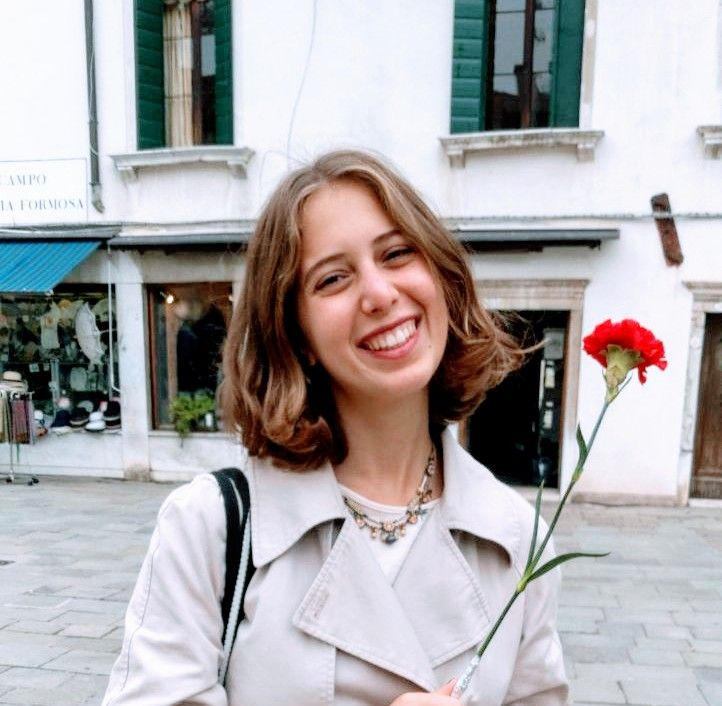
\includegraphics[width=30mm,height=30mm]{caterina}}
  \subfigure[Cristi Gutu]{
    
\includegraphics[width=30mm,height=30mm]{cristi}}
\end{figure}

\end{document}
